\section{Experimental methods}\label{supp:fields}\label{supp:metrics}
\subsection{Network, path sets, and demand settings}\label{supp:networks}
The public Sioux Falls network has $24$ nodes and $76$ directed arcs
\citep{tnfrc2024transportation}. All arcs belong to one cycle atom, hence
one compatibility class. The eight queries are the positive-demand OD pairs with the largest
published demands, with ties broken by ascending origin then destination
node ID. All happen to involve node $10$.
The queries are
$(10,16)$, $(16,10)$, $(10,11)$, $(10,15)$, $(15,10)$, $(10,17)$, $(11,10)$, $(17,10)$,
with published demands
$q_{\mathrm{base}}=(4400,4400,4000,4000,4000,3900,3900,3900)$ veh/h.
The attribution path changes these demands from $0.2q_{\mathrm{base}}$ to
$1.6q_{\mathrm{base}}$. Node IDs in the traffic experiments are one-based.
Flows retain the benchmark's approximate-hourly convention; one time unit
is $0.01$ h. A reported TSTT number is $\sum_e F_et_e(F_e)$ with $F_e$
in veh/h and $t_e$ in these time units: multiplying by $0.01$ gives the
hourly vehicle-hour total, without extrapolating to a day. All absolute
attribution and boundary-account numbers use the same convention.

For each OD we retain every loopless directed path if enumeration finishes
within $200$ paths, otherwise the ten shortest by free-flow cost (Yen's
algorithm, lexicographic edge-sequence tie breaking); no OD in this
network has a fully enumerated set under the threshold. All eight query
ODs use ten paths. The link--path incidence $\Delta$ and the matrix $A$
summing paths within each OD stay fixed, so $B\Delta=MA$ with the
appropriate full or study OD incidence matrix. The full-background
ten-path set has $5{,}280$ paths (ten per OD; the expanded set
$10{,}560$, twenty per OD); Appendix~\ref{supp:coverage} compares these
candidate-path models.

The path-exchange response space $T_{\mathrm{swap}}=\Delta\ker A$
(Appendix~\ref{app:membership}) has dimension $32$ in A with ten
paths for each study OD, and dimension $53$ in C with either ten or
twenty paths for every OD, equal to the full circulation-space
dimension $m-n+1=53$ (ranks computed from within-OD differences of
link--path incidence columns). Full background therefore spans the
complete circulation space through allowable path exchanges, while
the eight-OD path model spans a proper subspace.

The three demand settings share the same query endpoints. In setting A,
all other demands are zero. In setting B, assign all positive
background demands jointly with the study demands fixed at
$q^0=0.2q_{\mathrm{base}}=(880,880,800,800,800,780,780,780)$ veh/h in
the listed query order, freeze the resulting background link flows, and
re-equilibrate only the eight query ODs. In setting C, the other $520$
positive OD demands stay at published values while all $528$ ODs
re-equilibrate jointly at every path point and perturbation. TSTT and
its gradient use total link flows in B and C; setting C is a
full-background assignment with eight attribution queries, not an
attribution evaluation of all $528$ ODs.

\subsection{Equilibrium and its sensitivities}\label{supp:sue}
Unless stated otherwise, the fixed-path logit stochastic user equilibrium
(SUE) uses $\theta=1$ and BPR costs
$t_e(F_e)=t_{0,e}[1+0.15(F_e/c_e)^4]$. With $\Pi_j$ the path set,
\begin{equation}
h_p=q_jp_p(F),\quad
p_p(F)=\frac{\exp[-\theta(\Delta^\top t(F))_p]}
{\sum_{r\in\Pi_j}\exp[-\theta(\Delta^\top t(F))_r]},\quad
F=\Delta h.\label{eq:sueloading}
\end{equation}
This is the solution of
\[
\min_{h\ge0,\ Ah=q}\left\{
\sum_e\int_0^{(\Delta h)_e}t_e(s)ds+
\theta^{-1}\sum_p h_p(\log h_p-1)\right\}.
\]
For positive demands the feasible set is nonempty and compact and the
objective strictly convex. A zero path flow can be improved by transferring
mass from a positive path of the same OD, since the entropy change is
$\theta^{-1}\epsilon\log\epsilon+O(\epsilon)<0$; hence the minimizer is
positive. Its Hessian and sensitivity equations are
\begin{equation}
H=\Delta^\top\operatorname{diag}(t'_e)\Delta+
\theta^{-1}\operatorname{diag}(1/h_p)\succ0,\qquad
\begin{bmatrix}H&A^\top\\A&0\end{bmatrix}
\begin{bmatrix}\partial_jh\\\partial_j\nu\end{bmatrix}
=\begin{bmatrix}0\\\mathbf e_j\end{bmatrix}.
\label{eq:kkt_sensitivity}
\end{equation}
$A$ has full row rank, so the system is nonsingular and the implicit
function theorem gives a $C^1$ demand-to-flow map.

For background re-routing we solve the equivalent total-link-flow fixed
point $F=L(F,q)=\Delta\{q_jp_{\Pi_j}(F)\}_j$ by Newton steps with residual
line search. For frozen background the corresponding equation is
$F=F_{\mathrm{bg}}^0+\Delta_{\mathrm{study}}
\{q_jp_{\Pi_j}(F)\}_{j\in\mathrm{study}}$, where $F_{\mathrm{bg}}^0$
is fixed at the joint $q^0$ equilibrium. Costs and gradients use this
total $F$ in both equations. Every solution is checked against its path-loading
equation, with maximum absolute path-flow gap below $10^{-7}$ veh/h.
The $76$-dimensional implicit system avoids forming a dense path Hessian.
For an OD group $R$, define
\[
S_R=\theta\sum_{k\in R}\Delta_k
\left[\operatorname{diag}(h_k)-h_kh_k^\top/q_k\right]\Delta_k^\top,
\quad W=\operatorname{diag}(t'_e(F_e)),\quad S=S_{\mathrm{all}}.
\]
Differentiating the logit probabilities gives
$\partial_F L_R=-S_RW$. Consequently the total sensitivity satisfies
\begin{equation}
(I+SW)J_j=\Delta_jp_j,\qquad
J_j^{\mathrm{study}}=\Delta_jp_j-S_{\mathrm{study}}WJ_j,\qquad
J_j^{\mathrm{bg}}=-S_{\mathrm{bg}}WJ_j.
\label{eq:bg_sensitivity}
\end{equation}
Here ``study'' includes all eight queried ODs and ``background'' the
other $520$: $J_j=J_j^{\mathrm{study}}+J_j^{\mathrm{bg}}$,
$BJ_j^{\mathrm{study}}=\mu_j$, $BJ_j^{\mathrm{bg}}=0$, the study
term including responses of the other seven study ODs. The
decomposition uses one joint equilibrium, rather than sensitivities
at different congestion states.
For setting B the background flows have no derivative, so the same
implicit system uses $S=S_{\mathrm{study}}$, with
$J_j^{\mathrm{study}}=J_j$ and $J_j^{\mathrm{bg}}=0$.

Central finite differences independently re-solve Eq.~\eqref{eq:sueloading}
at $q\pm a_j\mathbf e_j$, $a_j=0.005q_{\mathrm{base},j}$ and
$a_j/2$; both steps are checked at every $\theta=1$ ten-path
re-routing integration point, the path-set and $\theta$ variations
add half-step checks for all eight columns at the path midpoint, and
the link Newton solver is compared against the successive-averages
background equilibria at their common eleven quadrature points.

\subsection{Conservative learned surrogate}\label{supp:protocol}
The zero-background surrogate parameterizes
$h_j=q_j\operatorname{softmax}(z(q)|_{\Pi_j})$, $f=\Delta h$.
The three hidden layers each have $128$ tanh units; the final layer is
linear. The logit head uses training-standardized demands while the raw
$q_j$ multiplies the shares, preserving nonnegative flow and exact
conservation. Computations use double precision.
Training targets are fixed-path logit-SUE assignments ($\theta=1$,
path fixed-point tolerance $10^{-6}$). The $2500/857/857$
training/validation/test split uses seed $20260820$, with demands
$q_j=q_{\mathrm{base},j}s_j$ and independent $s_j$ drawn from
LogNormal$(0,0.5^2)$ clipped to $[0.2,2]$.
Adam uses learning rate $0.003$, full-batch link-flow MSE, at most
$12{,}000$ steps, and validation every $50$ steps. The
minimum-validation-error state of each seed $0,\ldots,4$ supplies
the reported results, with automatic differentiation supplying their
Jacobians; the test split is used only for final reporting.

\subsection{Integration grids, connected boundaries, and cancellation diagnostics}\label{supp:quadrature}
All numerical integrations use composite trapezoids. The principal
learned zero-background results use $201$ quadrature points; direct
zero-background SUE and both background settings use $41$ in the main
table. Frozen background compares $11$ with $41$ points; re-routing
compares $11$, $21$, and $41$ nested points; the two near-balanced
queries add $81$ and $161$ nested points; the learned-versus-SUE
sensitivity comparison uses identical $41$-point grids, kept separate
from the $201$-point learned results (Appendix~\ref{supp:accuracy}).

Connected boundaries require both $G[U]$ and $G[V\setminus U]$ to be
connected on the underlying undirected graph, with $s_j\in U$, $t_j\notin U$.
Exact enumeration yields $10{,}270$--$13{,}253$ admissible sets for each
of the eight main study ODs, and $4{,}621$--$16{,}943$ for the six
additional queries of Appendix~\ref{supp:newod}.
Extrema of $-\mathbf1_U^\top B\widetilde C_j$ are evaluated by exact
enumeration, cross-checked against independent subset enumeration on
restricted neighborhoods; attaining sets are verified for membership
with values recomputed by direct summation. These are connected
regions, not claimed to be administrative boundaries.

For cancellation diagnostics define
$A_j=|\Delta q_j|\int_0^1\sum_{v\notin\{s_j,t_j\}}|(BD_\lambda J_j)_v|d\lambda$
and $\kappa_j=1-S_j/A_j$ when $A_j>0$. The triangle inequality gives
$0\le S_j\le A_j$. Both quantities use the specified $201$-point learned
grid and are summarized over the five seeds; checks on additional
path-set or dispersion models sample the demand-path midpoint and
endpoints.

\subsection{Six pre-specified queries away from node 10}\label{supp:newod}
The selection rule uses only published demands and free-flow
shortest-path times. Candidates are the positive-demand ODs whose origin
and destination both differ from node $10$; ranking them by demand and
splitting into three equal-count terciles, the minimum- and
maximum-free-flow-shortest-path OD within each tercile is selected, with
ties broken by ascending (origin, destination). The six queries are
$(7,18)$, $(1,19)$, $(4,5)$, $(1,15)$, $(6,8)$, and $(7,12)$, with
published demands $(200,300,500,500,800,700)$ veh/h and free-flow
shortest-path times $(2,22,2,23,2,19)$ time units; the joint
protocol, sensitivities, and boundary enumeration are as in
Section~\ref{subsec:newod}, with conservation checks at setting-C
floating-point levels (maximum path fixed-point residual
$1.6\times10^{-10}$ veh/h, midpoint implicit-versus-finite-difference
column error $2.6\times10^{-8}$, completeness $4.3\times10^{-7}$).

For the single-OD checks, let $\bar q=q^{\mathrm{base}}$ be the full
published demand vector over all $528$ positive-demand ODs. For each
focal query $j\in\{(1,19),(1,15),(7,12),(6,8)\}$, define
\begin{equation}
q^{(a)}=\bar q+(a q_j^{\mathrm{base}}-\bar q_j)e_j,
\qquad
q^{(b)}=\bar q+(b q_j^{\mathrm{base}}-\bar q_j)e_j,
\qquad
(a,b)\in\{(0.2,1.6),(0.9,1.1),(0.8,1.2)\},
\label{eq:singleodstates}
\end{equation}
where $e_j$ is the coordinate unit vector. All other $527$ demands,
including the other five selected queries, remain at their published
values $\bar q_{-j}$ along the segment. Direct equilibria and the learned
small-band checks use these same reference states. The setting-C solver,
path sets, and boundary definitions are unchanged; checks and interval
results are in Appendix~\ref{supp:newodaccuracy}. For each interval,
Eq.~\eqref{eq:edgeidentity} gives the attribution column from the two
endpoint equilibria alone.


\subsection{Anaheim network, equilibrium and predefined regions}\label{app:anaheimsettings}
Both network and demand files are the public Transportation Networks for Research Core Team Anaheim TNTP data \citep{tnfrc2024transportation}. The network header supplies free-flow times in minutes and capacities in vehicles per hour; all roads use the published BPR coefficient 0.15 and power 4. We use $t_e(F_e)=t_e^0[1+0.15(F_e/c_e)^4]$ and TSTT marginal weight $t_e^0[1+0.75(F_e/c_e)^4]$. The six study OD demands, ranked by descending base demand and then lexicographic OD, are $(4,2)$: 2106.7, $(1,2)$: 1365.9, $(2,4)$: 1271.4, $(3,2)$: 1237.9, $(25,4)$: 1232.4, $(25,2)$: 1232.3 vehicles per hour. They move jointly from 0.8 to 1.2 times base demand; all remaining positive demands stay at their published base values and retain endogenous route choice. Every OD uses ten loopless free-flow shortest routes from Yen's algorithm. Ties within $10^{-12}$ minutes are resolved by lexicographic edge-index sequence in the TNTP road order. Nodes 1--38 are centroids and cannot be intermediate route nodes; the first through node is 39. Logit scale $\theta=1$ minute$^{-1}$ applies to route travel time in minutes.
The edge Newton solver targets maximum loading residual below $10^{-8}$ vehicles per hour, uses at most 80 iterations and backtracking up to 30 halvings per step, and checks the original path loading residual below $10^{-7}$. Implicit derivatives solve the same fixed-point equation. Trapezoidal integration uses equally spaced states, with warm starts from a neighboring saved state. The 41-state refinement reuses all 21 old states and computes only the twenty new midpoints.
For each study OD, construct undirected BFS spanning trees rooted at each endpoint. At every visited node, traverse neighbors in increasing node-index order. Deleting each edge on the tree's endpoint path creates two connected parts; orient the region to contain the OD origin, and remove duplicate regions. This gives the selected connected family, not all connected separating regions. Sort the resulting node lists lexicographically to select first, middle and last regions for the mechanism comparisons. Free-flow weights are $t^0$ and congestion weights are the TSTT marginal weight minus $t^0$, at the same total-flow state for both study and background responses.

\subsection{Learning objectives and exact endpoint targets}\label{app:learning-objectives}
This identity suggests learning the reference's weighted demand response
where it affects spatial accounts. With training-only positive scales
$a_j$, the boundary term is
\begin{equation}
\mathcal L=\mathcal L_{\mathrm{flow}}+\lambda_J\mathcal L_{\mathrm{response}}
+\lambda_{\mathrm{cut}}\mathcal L_{\mathrm{boundary}},\qquad
\mathcal L_{\mathrm{boundary}}
=\frac1{NK}\sum_{q,j}\left[\frac{\mathcal K_j(h_j(q))}{a_j}\right]^2.
\label{eq:trainingobjective}
\end{equation}
The reference Jacobian is obtained from the existing implicit SUE
sensitivity system (Appendix~\ref{supp:sue}). We compare ordinary
flow supervision, flow plus response supervision, and the full objective.
Derivative supervision itself is established in Sobolev training
\citep{czarnecki2017sobolev}, including finite-difference derivative targets
\citep{yuan2022sobolev}; the network-derived target here selects the
part of weighted response error that changes boundary accounts.
A circulation in $\ker B$ is invisible to $\mathcal K_j$, so flow and
response losses remain necessary for the other attribution objectives.
The target matches the reference's actual response; it does not force
its true internal attribution divergence to zero or replace TSTT weights
with uniform weights. Equation~\eqref{eq:localboundarybound} is a path
inequality; finite training-point losses alone do not certify an entire
demand domain.


For the following finite-change statement, the outcome is explicitly separable:
\[
g(F)=(g_e(F_e))_{e\in E},\qquad T(F)=\sum_{e\in E}g_e(F_e).
\]
\begin{proposition}[exact finite-change boundary target]\label{prop:pairboundary}
Let $f^L,f^S$ and the edgewise outcome $g$ be continuously differentiable
on an open demand domain, and let $q^\pm=q\pm h e_j$ with their entire
segment in that domain. Put
\[
z_j^r=g(f^r(q^+))-g(f^r(q^-)),\qquad r\in\{L,S\}.
\]
For the attribution of this single-OD change,
\begin{equation}
\max_{U:s_j\in U,\ t_j\notin U}|\phi_j^L(U)-\phi_j^S(U)|
=\mathcal K_j(z_j^L-z_j^S).\label{eq:pairboundaryexact}
\end{equation}
If all sufficiently small single-coordinate changes have matching
accounts on every separating boundary at every point of the domain,
then $BD^LJ_j^L=BD^SJ_j^S$ throughout the domain. Integrating yields
matching boundary attribution columns for any joint demand path in that
domain (with the same columnwise path convention).
\end{proposition}
Appendix~\ref{app:pairproof} proves both statements. The first is an
exact finite-change target, whereas the pointwise response objective
optimizes the upper bound in Eq.~\eqref{eq:localboundarybound}; integrating
before taking $\mathcal K_j$ can retain cancellations. The second statement
requires a domain-wide local premise and is not a guarantee from finite
training data. With several ODs changing, the endpoint outcome difference
only identifies the sum of their attribution columns.

For sampled single-OD endpoint pairs, a direct training objective is
\begin{equation}
\mathcal L_{\mathrm{pair}}=\mathcal L_{\mathrm{flow}}
+\lambda_{\mathrm{edge}}\frac1N\sum_{(q,h,j)}
\frac{\|z_j^L-z_j^S\|_2^2}{b_j^2}
+\lambda_{\mathrm{cut}}\frac1N\sum_{(q,h,j)}
\left[\frac{\mathcal K_j(z_j^L-z_j^S)}{a_j}\right]^2,
\label{eq:pairobjective}
\end{equation}
with positive training-only scales $a_j,b_j$. The edge term controls
changes invisible to the boundary seminorm, whose kernel is $\ker B$.
Two reference endpoint equilibria supply $z_j^S$; training uses ordinary
parameter backpropagation through two predictions, without reference
Jacobian labels or input-Jacobian differentiation. Actual label-generation
and training costs must still be measured.

\subsection{Finite-change supervision: protocol and additional results}\label{app:pairs-v102}
All four methods continue each of the same five pretrained conservative models for 1,200 Adam updates (learning rate $3\times10^{-5}$, flow batch 32, query batch 8). The flow data and random minibatch sequences are shared. Each query has 64 training and 16 validation endpoint pairs. Pair centers are sampled independently, coordinatewise, from $[0.65,1.3]$ times baseline demand; half-widths are 2.5\% and 15\% of the queried baseline demand, equally represented. Only the queried demand changes within a pair; all background route shares remain responsive. Edge and boundary variants share exactly the same endpoint labels. Their weights are fixed at 1 and 0.01, respectively, without a new weight search. Training-only root-mean-square scales are used for each query.

All methods use the same 96 validation pairs every 100 updates. Among checkpoints whose mean relative flow error is at most 1.1 times the initial checkpoint's error, the minimum normalized boundary mean-square error is selected. If none qualifies, the minimum-flow-error checkpoint is retained. This fallback occurs for seeds 0, 2, and 3 of both endpoint variants; the flow threshold is therefore a selection preference, not a guarantee satisfied by every selected model. Test paths never enter selection.

For each path--query pair, let $e_j=\widetilde C_j^L-\widetilde C_j^S$ and $c_j=\widetilde C_j^S$. Column, system and boundary relative errors are respectively $\|e_j\|_2/\max(\|c_j\|_2,10^{-6})$, $|\mathbf1^\top e_j|/\max(|\mathbf1^\top c_j|,10^{-6})$, and $\mathcal K_j(e_j)/\max(\mathcal K_j(c_j),10^{-6})$. The absolute boundary error is $\mathcal K_j(e_j)$; geometric error replaces $\mathcal K_j$ in numerator and denominator with the maximum absolute account over the prescribed screenline family. Percentages multiply these ratios by 100.

The 24 prespecified test paths comprise six paths each with one, two, three, or six active queries. Cyclic combinations balance query participation within each group; paths include same-direction and mixed-direction changes of 15--30\% of baseline demand. Each path has 41 states. The flow column is the five-seed mean relative error on the original held-out demand-state split, not a new-path statistic. Other main-table statistics first average active queries and seeds within each path, then summarize the 24 paths; seeds do not increase the number of independent demand paths. The absolute lower bound on relative-error denominators is $10^{-6}$; the smallest observed reference boundary scale is 92.55. The largest reference completeness residual is $3.38\times10^{-8}$, and the largest learned-model residual is $2.98\times10^{-6}$. The single-OD fixed-budget comparison instead uses exact endpoint columns and no quadrature.



Additional path-median straight-screenline errors for flow, endpoint-edge, endpoint-edge-plus-boundary, and response supervision are respectively 7.91\%, 7.40\%, 7.97\%, and 5.81\%; flow-increment errors are 4.81\%, 4.89\%, 5.09\%, and 3.55\%. Across the five seeds, the ranges of mean boundary errors, giving equal weight to the 24 paths, are respectively $[13.36,24.12]\%$, $[12.29,17.69]\%$, $[12.27,20.58]\%$, and $[10.53,17.46]\%$.

The 960 new endpoint solves take 64.0\,s. The response implementation additionally solves all 480 pair centers and computes their sensitivities in 53.1\,s; 384 center derivatives enter training, while the 96 validation-center derivatives are unused but included in this measured cost. Test reference generation takes 74.4\,s. These figures exclude the existing flow dataset and pretrained checkpoints. Median continuation times per run, including initialization, validation, and model saving, are 246.0, 422.2, 275.1, and 297.1\,s in the above method order. Five seed workers run concurrently, with methods executed sequentially within each worker; total continuation wall time is 1,303.5\,s. Shared-machine contention and stage overlap prevent interpreting these per-method wall times as an algorithmic speed comparison. The corresponding median times for attribution and evaluation of all 24 paths, including forward passes, six directional derivatives, integration, and metric assembly, are 15.9, 15.8, 13.8, and 11.0\,s. Equal update counts do not imply equal reference-data or computational costs.

\section{Numerical accuracy and supporting results}\label{supp:numdetail}\label{supp:transrecords}
\subsection{Grid refinement, derivative, and solver checks}\label{supp:accuracy}
All differences here are observed numerical comparisons, not certified
bounds. Direct attribution-column differences are at most 0.178\% for
11 versus 41 states and $1.1\times10^{-4}\%$ for six-query/single-OD
41 versus 81 states. Near-zero accounts on 41/81/161 grids change by
less than $5\times10^{-6}$ percentage points (absolute $<0.01$); the
learned 201/801-state relative difference is $4.97\times10^{-6}$.
Implicit versus re-solved central-difference Jacobian errors are at most
$7.6\times10^{-5}$ (halved step $2.5\times10^{-5}$), or
$3.0\times10^{-8}$ for six-query/single-OD columns. Newton versus
successive-averages differences over 1,353 solves are at most
$1.31\times10^{-11}$. Maximum fixed-point and balance residuals are
$3.10\times10^{-8}$ and $1.82\times10^{-11}$ veh/h. Scalar completeness
relative discrepancies are at most $3.36\times10^{-5}$ for
frozen/re-routing settings and $1.9\times10^{-7}$ for single-OD checks.
Per-edge endpoint checks give relative column errors
$7.7\times10^{-8}$--$1.1\times10^{-6}$ and maximum entry residuals
$5.4\times10^{-4}$--$1.6\times10^{-2}$ TSTT units. Per-query records
remain in the arrays. The direct $(10,16)$ account change is 24.80\%
on its 41-state grid; Figure~\ref{fig:respfield} uses the seed-zero
learned model on 201 states (24.8\%).

\subsection{Normalization, cancellation, and sensitivity}\label{supp:additional}
\paragraph{Error-metric definitions.}
The surrogate test flow error is, within each seed, the mean over the
$857$ test demands of
$\|f(q)-F^{\mathrm{SUE}}(q)\|_2/\|F^{\mathrm{SUE}}(q)\|_2$, reported
as the median over the five seeds; Jacobian column errors
$\|J_j^{\mathrm{learned}}-J_j^{\mathrm{SUE}}\|_2/\|J_j^{\mathrm{SUE}}\|_2$
are pooled over the $5\times41\times8$ seed--point--OD columns;
attribution-column errors use the per-column norm over the $40$
seed--OD columns on the common $41$-point grid.

\paragraph{Same-path flow, sensitivity, and boundary-account errors.}
The test-split flow error is not paired with the Jacobian
comparison; re-summarized on the same $41$ zero-background quadrature
points for each seed (median / 95th percentile / maximum, percent):
flow error $0.136$ / $0.682$ / $1.331$; Jacobian column error
$0.516$ / $3.903$ / $9.562$ (maximum at seed $3$, OD $(16,10)$,
$\lambda=0.925$; $5\times41\times8$ seed--point--OD units);
attribution-column
errors median $0.349\%$, maximum $1.80\%$; and
$E_j^{\mathrm{cut}}$, which evaluates both models' accounts at every
connected boundary of a query's family on the same path
(the unrestricted-family counterpart is virtually identical), at
$0.204$ / $0.650$ / $1.739$ ($40$ seed--OD units; largest connected
error at OD $(16,10)$, seed $3$).

Table~\ref{tab:origin_denominators} supplies the per-query absolute
origin-cut denominators for Table~\ref{tab:cutspreadperod}. The
setting-C link sums $C_j$ span $2.078$--$4.282\times10^5$ TSTT units,
exceeding origin-cut accounts by factors of $1.01$--$2.37$; their sum
matches the endpoint TSTT change within $2.3\times10^{-5}$ relative.
\begin{table}[pos=htbp]
\caption{Absolute direct-SUE origin-cut accounts
$|\phi_j(\{s_j\})|$, in TSTT units, for the eight queries in
Table~\ref{tab:cutspreadperod}. A, B, C use their respective
$41$-point columns; entries rounded to one decimal.}
\label{tab:origin_denominators}
\small
\begin{tabular*}{\tblwidth}{@{\extracolsep{\fill}}lrrr}
\toprule
OD & A & B & C\\
\midrule
$(17,10)$ & $29{,}372.1$ & $249{,}729.2$ & $224{,}954.3$ \\
$(10,17)$ & $46{,}977.2$ & $317{,}861.9$ & $245{,}178.7$ \\
$(16,10)$ & $41{,}994.3$ & $352{,}858.5$ & $180{,}671.5$ \\
$(10,16)$ & $57{,}468.9$ & $405{,}374.2$ & $272{,}743.2$ \\
$(15,10)$ & $33{,}859.4$ & $226{,}878.2$ & $201{,}351.2$ \\
$(10,15)$ & $34{,}056.4$ & $258{,}682.3$ & $232{,}160.6$ \\
$(10,11)$ & $28{,}807.1$ & $339{,}651.4$ & $202{,}928.2$ \\
$(11,10)$ & $28{,}010.4$ & $324{,}427.0$ & $204{,}802.3$ \\
\bottomrule
\end{tabular*}
\end{table}

The node breakdown in Table~\ref{tab:bgdecomp} complements the fixed
boundary comparison of Section~\ref{subsec:bgsplit}.
\begin{table}[pos=htbp]
\caption{Signed node divergence in the re-routing setting, at the
same joint equilibrium state and total-flow gradient at each of the
$41$ quadrature points (study includes all eight query ODs; TSTT
units of Appendix~\ref{supp:networks}; entries rounded independently,
so a component sum may differ from the rounded total in its last
digit).}
\label{tab:bgdecomp}
\small
\begin{tabular*}{\tblwidth}{@{\extracolsep{\fill}}llrrr}
\toprule
OD & Node & Study & Background & Total\\
\midrule
$(10,16)$ & $15$ & $-973.1$ & $49,103.4$ & $48,130.3$ \\
$(10,16)$ & $8$ & $9.6$ & $42,102.7$ & $42,112.3$ \\
$(10,16)$ & $20$ & $0.2$ & $41,805.4$ & $41,805.6$ \\
$(10,11)$ & $5$ & $0.5$ & $35,952.1$ & $35,952.6$ \\
$(10,11)$ & $12$ & $0.0$ & $-23,858.1$ & $-23,858.1$ \\
$(10,11)$ & $9$ & $-0.2$ & $-18,557.6$ & $-18,557.7$ \\
\bottomrule
\end{tabular*}
\end{table}

For the learned zero-background low-range group, five-seed median pointwise
imbalance budgets $100A_j/|\phi_j(\{s_j\})|$ lie between $0.22\%$ and
$0.95\%$, versus $26.85$--$59.71\%$ for the high group; the low-group
median cancellation factors are at most $0.313$ (one seed reaches
$\kappa=0.852$), so small pointwise imbalance mainly limits the
low-group range, while the high group's median $\kappa$ is below
$8\times10^{-5}$.

Zero-background route-choice dispersion checks at $\theta\in\{0.5,1,2\}$
(eleven-point direct-SUE calculations) retain the large/small
separation --- large ranges $27$--$64\%$, the others below $9.4\%$.

\subsection{Full-background six-query surrogate validation}\label{supp:fullbgsurrogate}
The six-query conservative surrogate predicts shares over all 5,280
paths, with the architecture of Appendix~\ref{supp:protocol}, dataset
seed 20261025 and batch size 256. Its 4,214 target solves have maximum
path residual $3.5\times10^{-8}$; learned conservation residual is at
most $3.6\times10^{-11}$. Held-out flow error is 0.040\% (seed median;
range 0.035--0.056\%). On the 41 common path states, flow errors are
0.037--0.065\%, but increment errors are 5.0--7.0\% against a reference
increment norm 2,982.7 (2.7\% of flow level). Median column errors are
81.2\% for $(7,18)$, 31.1\% for $(4,5)$ and 7.4--11.8\% for the
others. System contribution errors reach 14.7\% and 10.3\% for those
two queries, versus at most 3.7\% for the sign-crossing queries.
Table~\ref{tab:fullbgsurrogate} retains extrema and boundary errors;
learned column completeness is within $6\times10^{-6}$ relative.

An exact two-term split of \eqref{eq:Cdef} ($L$/$S$: learned/direct)
identifies where this error arises:
\begin{equation}
\widetilde C_{:,j}^{L}-\widetilde C_{:,j}^{S}
=\Delta q_j\int_0^1(D_\lambda^{L}-D_\lambda^{S})J_j^{S}\,\mathrm{d}\lambda
+\Delta q_j\int_0^1D_\lambda^{L}(J_j^{L}-J_j^{S})\,\mathrm{d}\lambda,
\label{eq:coldecomp}
\end{equation}
satisfied entrywise within $10^{-10}$ TSTT units. The weight-shift
term has querywise median norm at most 0.2\% of the reference column;
the response term is larger in every one of the thirty seed--query
units. Their norm sum is at most 1.04 times the realized error norm.
Signed scalar terms can cancel, so these norms are not additive shares.
Small-band endpoint columns have 4.8--15.9\% error and system values
within 2.7\% of reference, while every seed retains the reported signs.

\subsection{Sensitivity to candidate paths and route-choice dispersion}\label{supp:coverage}
The path-set comparison expands all $528$ OD sets to twenty
candidates each (the first ten unchanged), with demands, BPR
functions, $\theta=1$, and $41$ quadrature points fixed: across the
eight queries, absolute unrestricted and connected ranges change by
at most $0.977\%$ and $1.011\%$, with the three largest
internal-node terms keeping their ordered node IDs (moving at most
$1.43\%$). The $\theta\in\{0.5,2\}$ check splits the specified
$(10,16)$ boundary difference into study/background components
$-7{,}404.9$/$-2{,}371.5$ at $\theta=0.5$ and $+115.3$/$+235.7$ at
$\theta=2$; for all three additional models, implicit derivative
columns match re-solved half-step central differences at the
demand-path midpoint (maximum $0.00249\%$, completeness gap
$2.85\times10^{-5}$).

\subsection{Six-query interval, mechanism, boundary-family, and
scenario checks}\label{supp:newodaccuracy}


\textbf{Extremal ranges and negative shares.}
Unrestricted extrema follow the closed form \eqref{eq:cutextrema},
connected extrema the same enumeration as the connected ranges
(Table~\ref{tab:newodinterval}); the negative shares in
Section~\ref{subsec:newod} are exact counts over the connected
families ($4{,}621$--$16{,}943$ admissible sets per query), and all
displayed values come from the $41$-point columns.

\begin{table}[pos=tbh]
\caption{Minimum--maximum boundary-account ranges for the three
sign-crossing queries of Table~\ref{tab:newod}, in TSTT units
(Appendix~\ref{supp:networks}), rounded to integers. Baseline:
unrestricted extrema (closed form \eqref{eq:cutextrema}; connected
extrema in Table~\ref{tab:newod}); next four rows: connected
ranges under the model-setting changes and the single-OD
$0.2\to1.6$ re-run (unrestricted intervals within $1\%$ of the
baseline row); last two: small-interval bands, with $C_j$ positive
($+7{,}202$ to $+33{,}734$ across the three queries) and the control
$(6,8)$ positive ($[5{,}079,\ 9{,}623]$ and $[10{,}157,\ 19{,}246]$;
single-OD $[35{,}352,\ 66{,}861]$).}
\label{tab:newodinterval}
\small
\begin{tabular*}{\tblwidth}{@{\extracolsep{\fill}}lrrr}
\toprule
Range & $(1,19)$ & $(1,15)$ & $(7,12)$\\
\midrule
Baseline ($10$ paths, $\theta=1$): unrestricted & $[-19{,}116,\ 26{,}696]$ & $[-16{,}240,\ 44{,}137]$ & $[-45{,}241,\ 61{,}650]$\\
\addlinespace
Twenty paths, $\theta=1$: connected & $[-13{,}451,\ 24{,}276]$ & $[-8{,}329,\ 40{,}644]$ & $[-17{,}728,\ 59{,}452]$\\
Ten paths, $\theta=0.5$: connected & $[-13{,}024,\ 24{,}064]$ & $[-8{,}107,\ 39{,}933]$ & $[-17{,}633,\ 60{,}476]$\\
Ten paths, $\theta=2$: connected & $[-13{,}016,\ 24{,}411]$ & $[-8{,}233,\ 40{,}892]$ & $[-19{,}587,\ 61{,}647]$\\
Single-OD $0.2\to1.6$: connected & $[-13{,}608,\ 24{,}414]$ & $[-8{,}359,\ 40{,}745]$ & $[-17{,}580,\ 60{,}006]$\\
Single-OD $\pm10\%$ band ($0.9\to1.1$): connected & $[-1{,}947,\ 3{,}494]$ & $[-1{,}201,\ 5{,}838]$ & $[-2{,}517,\ 8{,}608]$\\
Single-OD $\pm20\%$ band ($0.8\to1.2$): connected & $[-3{,}895,\ 6{,}988]$ & $[-2{,}402,\ 11{,}677]$ & $[-5{,}035,\ 17{,}215]$\\
\bottomrule
\end{tabular*}
\end{table}

\textbf{Connected minimum and divergence decomposition.}
Table~\ref{tab:negmech} reports, for each sign-crossing query, the
connected minimizing boundary $U_-$ at the baseline setting: its
account, and the interior divergence sum
$\phi_j(\{s_j\})-\phi_j(U_-)$, decomposed as the table caption
specifies, at the same joint state and gradient as the reported
columns (additivity $\le1.2\times10^{-10}$).
By Eq.~\eqref{eq:cutgap}, the negative divergence captured inside
$U_-$ ($4{,}664.9$, $6{,}960.1$, and $19{,}811.5$ for the three
queries) covers $83\%$, $88\%$, and $72\%$ of the gaps
$\phi_j(U_-)-\phi_j^{\min}$, while the captured positive divergence
($19{,}938.0$, $18{,}194.2$, $46{,}901.4$) is $95.5\%$, $94.8\%$,
and $85.7\%$ of the query totals. The sign change arises
differently across queries: study response
dominates for $(1,19)$ (largest node $15$: own $+14{,}464.0$),
study- and background-dominated nodes share the sign for $(1,15)$,
and both contribute about equally for $(7,12)$ (node $8$).
The extremal node sets (one-based node IDs) are
$U_-(1,19)=\{1,2,6,7,8,9,15,16,18,20,21,22,24\}$ and
$U_+(1,19)=\{1,2,3,4,5,6,10,11,12,13,14,22,23\}$;
$U_-(1,15)=\{1,2,6,7,8,9,16,17,18,19,20,21,24\}$ and
$U_+(1,15)=\{1,2,3,4,5,6,10,11,12,13,14,22,23\}$;
$U_-(7,12)=\{1,2,3,4,5,6,7,8,9,10,11,14,17,19,23\}$ and
$U_+(7,12)=\{7,8,9,15,16,18,20,21,22,24\}$.

\begin{table}[pos=tbh]
\caption{Connected minimizing boundary $U_-$ at the baseline setting
for the three sign-crossing queries, in TSTT units. Interior is the
divergence sum over $U_-\setminus\{s_j\}$, decomposed into the query's
own response, the other five query ODs, and the background response;
node sets are the one-based lists in the preceding paragraph. Entries
are rounded independently.}
\label{tab:negmech}
\small
\begin{tabular*}{\tblwidth}{@{\extracolsep{\fill}}lrrrrrr}
\toprule
OD & $\phi_j(\{s_j\})$ & $\phi_j(U_-)$ & Interior & Own OD & Other query & Background\\
\midrule
$(1,19)$ & $1{,}771.6$ & $-13{,}501.6$ & $15{,}273.1$ & $19{,}480.9$ & $-59.4$ & $-4{,}148.3$ \\
$(1,15)$ & $2{,}948.1$ & $-8{,}286.0$ & $11{,}234.1$ & $7{,}856.9$ & $-26.7$ & $3{,}404.0$ \\
$(7,12)$ & $9{,}473.8$ & $-17{,}616.2$ & $27{,}089.9$ & $14{,}002.3$ & $-3.2$ & $13{,}090.8$ \\
\bottomrule
\end{tabular*}
\end{table}

\textbf{Neighbourhood families.}
Use undirected hop distance or shortest free-flow distance from the origin
(minimum weight over parallel arcs). Include nodes at each attained radius,
stop before including the destination, and retain only two-sided connected
regions. Table~\ref{tab:neighbourhoods} reports all family ranges; all are
positive with minima at the origin cut. For short-path queries $(7,18)$,
$(4,5)$ and $(6,8)$, only that cut is admissible. The thirteen-node
free-flow ball at radius 16 for $(1,19)$ is
$\{1,2,3,4,5,6,7,8,9,11,12,13,24\}$, with account $+10{,}756.0$.

\begin{table}[pos=htbp]
\caption{Origin-centred neighbourhood accounts, baseline six-query setting C
(TSTT units). Counts are distinct admissible node sets within each family;
sets shared by the two families are counted in each row.}\label{tab:neighbourhoods}
\small
\begin{tabular*}{\tblwidth}{@{\extracolsep{\fill}}llrrr}
\toprule OD & Neighbourhood & Count & Minimum & Maximum\\\midrule
$(1,19)$ & Hop distance & 6 & $1,771.6$ & $15,803.5$\\
$(1,19)$ & Free-flow time & 13 & $1,771.6$ & $15,803.5$\\
$(1,15)$ & Hop distance & 5 & $2,948.1$ & $26,602.0$\\
$(1,15)$ & Free-flow time & 14 & $2,948.1$ & $26,602.0$\\
$(7,12)$ & Hop distance & 4 & $9,473.8$ & $31,524.1$\\
$(7,12)$ & Free-flow time & 9 & $9,473.8$ & $32,139.4$\\
\bottomrule\end{tabular*}\end{table}

\textbf{Straight screenlines.}
Coordinates use an equirectangular frame (longitude scaled by the cosine
of mean latitude). Section~\ref{sec:scan}'s 36-direction construction,
with duplicate regions removed, gives 35, 152, 32, 123, 23 and 148
regions in Table~\ref{tab:newod} order. All accounts agree with direct
incidence aggregation below $10^{-9}$. Refining directions from
$5^\circ$ to $1^\circ$ leaves both negative minima unchanged; negative
shares change from 1.3\% to 1.8\% for $(1,19)$ and 6.8\% to 6.2\%
for $(7,12)$. Other queries stay positive; only $(7,18)$'s minimum
changes, from 642.4 to 641.4.

\textbf{Model-setting checks.}
Re-solving the protocol of Appendix~\ref{supp:newod} under twenty
candidate paths per OD and $\theta\in\{0.5,2\}$ at ten paths gives
the ranges of Table~\ref{tab:newodinterval} ($C_j$ within $3.9\%$);
solver and finite-difference checks match
Appendix~\ref{supp:newod} levels.

\textbf{Single-OD demand changes.}
Each single-OD demand path ($0.2\to1.6$ of published demand)
re-solves the setting-C protocol with one moving coordinate. For the
three crossing queries the connected ranges (Table~\ref{tab:newodinterval},
single-OD row) still straddle zero, their extrema attained by exactly
the joint-scenario sets $U_-$ and $U_+$ (changes at most $0.9\%$ and
$0.5\%$; unrestricted intervals within $1\%$ of the joint baseline)
and the contributions stay positive ($C_j=50{,}322.2$, $77{,}672.6$,
$117{,}476.8$); the control $(6,8)$ remains sign-consistent
($C_j=74{,}176.1$, connected range in the caption). The
small-interval bands (Table~\ref{tab:newodinterval}, last two rows)
follow the same protocol, the $41$-point check ($(1,19)$,
$0.8\to1.2$) reproducing the endpoint column to $1.3\times10^{-5}$
TSTT units per edge.

\begin{figure}[pos=htbp]
\centering
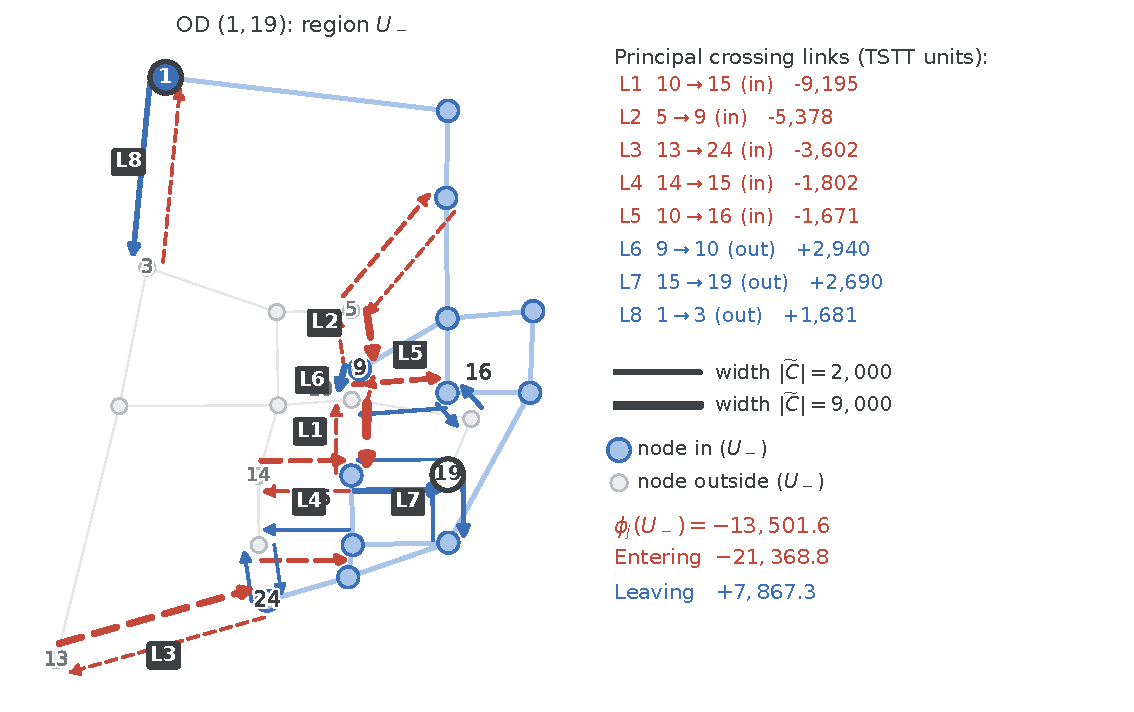
\includegraphics[width=0.95\linewidth]{../figures/fig_negmech_v102.pdf}
\caption{The connected minimizing region $U_-$ for OD $(1,19)$
(setting C, six-query protocol). Shaded nodes form $U_-$ (origin
node $1$ ringed; destination $19$ outside). Crossing-link arrows keep
the link direction; width scales with $|\widetilde C_{e,j}|$, and
colour and style encode the signed contribution to $\phi_j(U_-)$,
$a_{e,j}=\sigma_e\widetilde C_{e,j}$ ($\sigma_e=+1$ leaving, $-1$
entering; solid blue positive, dashed red negative), so a positive
attribution on an entering link appears red. The side panel lists, in
TSTT units, the five largest negative and three largest positive
contributions among the $26$ crossing links
($\mathrm{L}1$--$\mathrm{L}5$ negative, $\mathrm{L}6$--$\mathrm{L}8$
positive, ``(in)''/``(out)'' marking entering and leaving links),
with the width scale and the membership legend.}
\label{fig:negmech}
\end{figure}
\textbf{Endpoint identity checks.}
Appendix~\ref{supp:accuracy} reports the per-edge
endpoint-identity errors and their relation to completeness gaps on
these same demand paths.

\FloatBarrier
\subsection{Baseline surrogate envelopes}\label{supp:baselineenvelopes}
\begin{table}[pos=htbp]
\caption{Full-background surrogate validation on the identical
$41$-state path of the six-query protocol (setting C; TSTT units;
contributions and extrema rounded to integers, errors to one
decimal). $C_j^{\mathrm{learned}}$ and the connected extrema:
across-seed envelopes of per-model values (direct-SUE values in
Table~\ref{tab:newod}). Last two columns: five-seed
\emph{median} of the largest connected-boundary disagreement
$\epsilon_j^{\mathrm{cut}}$, in absolute units and as a percentage of
the direct connected span.}
\label{tab:fullbgsurrogate}
\small
\begin{tabular*}{\tblwidth}{@{\extracolsep{\fill}}lrrrrr}
\toprule
& & \multicolumn{2}{c}{Connected extrema: across-seed ranges}\\
\cmidrule(lr){3-4}
OD & $C_j$: across-seed envelope & per-model minima & per-model maxima & $\epsilon^{\mathrm{cut}}$ (med.) & $\epsilon^{\mathrm{cut}}$/span (med., \%)\\
\midrule
$(7,18)$ & $[574,\ 681]$ & $[335,\ 521]$ & $[907,\ 1{,}299]$ & $397.5$ & $522.5$ \\
$(1,19)$ & $[49{,}929,\ 51{,}452]$ & $[-13{,}911,\ -13{,}334]$ & $[23{,}683,\ 23{,}948]$ & $1{,}567.4$ & $4.2$ \\
$(4,5)$ & $[2{,}535,\ 2{,}934]$ & $[1{,}654,\ 2{,}148]$ & $[2{,}946,\ 3{,}546]$ & $1{,}050.8$ & $99.5$ \\
$(1,15)$ & $[77{,}416,\ 80{,}233]$ & $[-7{,}717,\ -6{,}766]$ & $[39{,}473,\ 40{,}076]$ & $2{,}187.3$ & $4.5$ \\
$(6,8)$ & $[73{,}565,\ 75{,}224]$ & $[36{,}412,\ 37{,}631]$ & $[66{,}892,\ 67{,}762]$ & $2{,}163.2$ & $6.9$ \\
$(7,12)$ & $[116{,}562,\ 118{,}706]$ & $[-17{,}084,\ -15{,}198]$ & $[59{,}965,\ 61{,}169]$ & $4{,}111.3$ & $5.3$ \\
\bottomrule
\end{tabular*}
\end{table}



\subsection{Fixed-screenline surrogate comparisons}\label{supp:screenlinelearned}
\begin{table}[pos=htbp]
\caption{Fixed straight screenlines: reference minimum and the five frozen flow-supervised surrogates at that same screenline (TSTT units). The last column gives the largest error over the screenline family, as an across-seed range.}
\label{tab:screenlinelearned}
\small\begin{tabular*}{\tblwidth}{@{\extracolsep{\fill}}lrrr}\toprule
OD & Reference minimum & Learned account: seed range & Maximum screenline error: seed range\\\midrule
$(7,18)$ & 642.4 & $[576.9,\ 789.8]$ & $[141.0,\ 269.4]$ \\
$(1,19)$ & -2766.6 & $[-3886.6,\ -3365.1]$ & $[857.9,\ 1430.8]$ \\
$(4,5)$ & 2652.3 & $[2301.7,\ 2918.8]$ & $[438.0,\ 648.3]$ \\
$(1,15)$ & 511.1 & $[732.8,\ 2068.2]$ & $[1140.6,\ 2553.0]$ \\
$(6,8)$ & 45230.2 & $[46431.5,\ 47218.3]$ & $[1276.2,\ 1988.1]$ \\
$(7,12)$ & -2967.3 & $[-2810.4,\ -1916.6]$ & $[1736.8,\ 2499.2]$ \\
\bottomrule\end{tabular*}\end{table}


\paragraph{Sign preservation.}\label{subsec:precision}
All five baseline seeds retain the three connected-family sign crossings
and positive system contributions. At the fixed reference extrema,
$m_j=\min\{-\phi_j^S(U_-),\phi_j^S(U_+)\}-\epsilon_j^{\rm conn}$
is positive, with smallest value 5519 TSTT units. This verifies sign
preservation without implying accurate column magnitudes.

At the fixed direct-model minimizing screenline, every baseline seed
retains the negative sign for both queries: $(1,19)$ gives
$[-3886.6,-3365.1]$ against the reference $-2766.6$, and $(7,12)$
gives $[-2810.4,-1916.6]$ against $-2967.3$. Their largest family-wide
errors across seeds are $1430.8$ and $2499.2$, below the respective
reference sign margins. These are screenline-specific certificates;
they supplement the separate connected-family result above
(Appendix~\ref{supp:screenlinelearned}).


The eight-query path-set and dispersion checks are collected in
Appendix~\ref{supp:coverage}. Boundary variation persists, although
the specified $(10,16)$ comparison $\{10\}\to\{10,17\}$ changes sign
across $\theta$; these are different fixed-path models, not convergence
to unrestricted SUE.

\subsection{Final learning comparison: budgets and groups}
Tables~\ref{tab:pair-budget-v102} and~\ref{tab:pair-groups-v102} report the fixed-budget and path-group breakdowns of the final comparison.
\begin{table}[t]\centering\small
\caption{Fixed-budget endpoint boundary error (\%) on six independent single-OD test paths. Seeds are averaged within each path before taking the path median.}
\label{tab:pair-budget-v102}
\begin{tabular}{lrrr}\toprule Method & 300 updates & 600 updates & 1,200 updates\\\midrule
Flow & 4.40 & 4.13 & 3.97\\
Flow + endpoint edge & 4.47 & 4.35 & 4.16\\
Flow + endpoint edge + cut & 4.51 & 4.38 & 4.17\\
Flow + response & 3.52 & 3.16 & 3.02\\
\bottomrule\end{tabular}\end{table}

\begin{table}[t]\centering\small
\caption{Mean unrestricted boundary error (\%) by number of active queries. Each group contains six independent paths, each balanced across queries.}
\label{tab:pair-groups-v102}
\begin{tabular}{lrrrr}\toprule Method & One OD & Two ODs & Three ODs & Six ODs\\\midrule
Flow & 14.34 & 18.24 & 19.71 & 19.80\\
Flow + endpoint edge & 11.11 & 15.72 & 16.06 & 18.93\\
Flow + endpoint edge + cut & 13.08 & 16.65 & 15.09 & 19.56\\
Flow + response & 12.67 & 16.30 & 13.45 & 13.73\\
\bottomrule\end{tabular}\end{table}


\subsection{Input-stratified OD coverage}\label{sec:coverage}
We select queries using only the published positive OD demand and directed free-flow shortest-path time. Each attribute is divided at its empirical tertiles, keeping ties in the lower group. In each of the nine cells, OD pairs are ordered lexicographically and the pairs at zero-based positions $\lfloor N/3\rfloor$ and $\lfloor2N/3\rfloor$ are retained. Empty cells remain empty and a singleton is retained once. This yields 18 queries from 528 positive demands. For each query, only its demand moves from $(1-a)q_j$ to $(1+a)q_j$, $a\in\{0.1,0.2\}$; all other demands remain at their published levels with endogenous route choice. Four endpoint equilibria per query give the exact single-OD edge attribution by Eq.~\eqref{eq:edgeidentity}, avoiding quadrature. The geometric family uses the same 36 pre-specified directions and connected-side filter as the screenline experiment.
\begin{table}[t]\centering\small
\caption{All input-stratified queries. Entries are geometric-account spreads for $\pm10\%$ and $\pm20\%$ intervals and their ratios to the exact unrestricted spread. Absolute values use the Sioux Falls cost units. No query is removed based on its attribution.}\label{tab:coverage}
\begin{tabular}{lrrrr}\toprule
OD & $S_{\rm geo}^{10}$ & $S_{\rm geo}^{20}$ & $S_{\rm geo}^{10}/S_{\rm all}^{10}$ & $S_{\rm geo}^{20}/S_{\rm all}^{20}$\\\midrule
(4,3) & 53.0 & 105.9 & 0.353 & 0.353\\
(12,3) & 4.8 & 9.5 & 0.417 & 0.417\\
(6,1) & 816.1 & 1632.1 & 0.651 & 0.651\\
(15,6) & 2009.1 & 4018.1 & 0.672 & 0.672\\
(6,21) & 1176.4 & 2352.8 & 0.668 & 0.668\\
(18,14) & 889.5 & 1778.9 & 0.511 & 0.511\\
(8,4) & 7235.2 & 14470.6 & 0.646 & 0.646\\
(19,8) & 3266.6 & 6533.2 & 0.374 & 0.374\\
(11,6) & 2434.9 & 4869.9 & 0.626 & 0.626\\
(16,2) & 4366.2 & 8732.3 & 0.545 & 0.545\\
(8,21) & 1730.7 & 3461.5 & 0.424 & 0.424\\
(14,8) & 3318.4 & 6636.8 & 0.495 & 0.495\\
(11,15) & 5054.3 & 10108.8 & 0.337 & 0.337\\
(17,9) & 6509.7 & 13037.1 & 0.696 & 0.695\\
(10,12) & 11713.3 & 23426.2 & 0.539 & 0.539\\
(13,10) & 14211.4 & 28426.4 & 0.667 & 0.667\\
(1,10) & 9336.8 & 18673.5 & 0.603 & 0.603\\
(10,1) & 9428.5 & 18856.8 & 0.606 & 0.606\\
\bottomrule\end{tabular}\end{table}
The median geometric-to-unrestricted spread ratios are 0.574 and 0.574 for the two widths. These results describe this fixed input-stratified sample; they are not a probability sample of all demand conditions. Endpoint differences identify total edge accounts, but do not identify the same-state study/background response decomposition. That decomposition is evaluated separately in the mechanism experiments.

\subsection{Supplementary pointwise-supervision comparisons}\label{app:legacy-learning}\label{app:learning-protocol}\label{app:calibration-protocol}
Two earlier comparisons use the same five full-background flow-trained
models, original data split and three-layer 128-unit tanh architecture
with 5,280 path logits. All continuation runs use 600 Adam updates,
learning rate $3\times10^{-5}$, flow batches of 32 and response batches
of eight, cycling six queries. Reference derivatives at 256 training
states use sampling seed 20261029; 64 additional derivative states are
reserved for validation. Flow scales are $0.01$ times edgewise training
root-mean-square flows; response and boundary scales are querywise
training root-mean-square column norms and $\mathcal K_j$ values,
respectively. All losses average squared normalized errors. Model
response derivatives are obtained by automatic differentiation.

The fixed-coefficient comparison sets both added loss coefficients to one,
uses shared seed-specific flow minibatches, and retains the final update
without selection. Four test paths, generated before training with seed
101029, have one, two, three and six active queries, mixed directions and
baselines in $[0.65,1.3]$ times published demands. Each has 41 quadrature
states. Attribution metrics summarize 60 active query--path--seed units,
flow metrics five seeds and increment metrics 20 path--seed pairs.
Boundary errors divide by $\mathcal K_j(\widetilde C^S_{:,j})$; column,
system and increment errors divide by the corresponding reference norm
or absolute value. These descriptive units are not treated as independent
paths for inferential statistics.
\begin{table}[t]
\centering\small
\caption{Equal-update continuation from five flow-trained checkpoints on four independent demand paths. Entries are medians over 60 active query--path--seed combinations, except flow (five seeds, held-out split) and increment error (20 path--seed pairs). Boundary error uses all separating cuts and is normalized by the corresponding maximum absolute reference account.}
\label{tab:structured-learning}
\begin{tabular}{lrrrrrr}\toprule
Method & Flow (\%) & Increment (\%) & Column (\%) & System (\%) & Cut abs. & Cut (\%)\\\midrule
Original & 0.04 & 5.18 & 14.11 & 2.08 & 260.55 & 9.93\\
Flow continuation & 0.03 & 5.34 & 12.29 & 1.48 & 268.81 & 9.98\\
Flow + response & 0.03 & 5.48 & 11.92 & 1.65 & 283.64 & 9.64\\
Flow + response + boundary & 0.12 & 14.07 & 32.01 & 1.97 & 708.35 & 22.25\\
\bottomrule\end{tabular}
\end{table}

Adding the boundary term increases pooled boundary error from 9.64\% to
22.25\%, although it improves 14/15 $(7,18)$ units and 8/10 $(4,5)$
units; the other query groups worsen. Reference labels and test paths
require 83.3\,s. Median continuation times are 105.6, 184.8 and 244.5\,s
for flow, response and boundary methods. Maximum conservation residual
is $4.6\times10^{-11}$; relative quadrature completeness discrepancy is
at most $5.1\times10^{-6}$.

The calibrated comparison selects $\lambda_{\rm cut}$ from
$\{0.001,0.01,0.1\}$ on seed zero, using the 64 reserved validation
states. It minimizes normalized boundary-response mean square subject
to validation flow error at most 110\% of the response comparator.
The chosen coefficient is then applied to all five seeds, reusing its
seed-zero fit: seven structural fits in total. Validation flow errors
are $0.0610\%$ for the response comparator and $0.0611\%$, $0.0631\%$,
$0.0804\%$ for the candidates; corresponding boundary-response mean
squares are $0.7040$, $0.6852$, $0.6097$, $0.4532$. Thus $0.1$ fails
the flow criterion and $0.01$ is selected. This additional search budget
precludes an equal-search advantage claim. Four new test paths use seed
101030 and the same active-query templates, with evaluation after
selection; the original paths remain diagnostic data.
\begin{table}[t]
\centering\small
\caption{Exploratory validation-calibrated continuation ($\lambda_{\mathrm{cut}}=0.01$), tested on four new independent demand paths (seed 101030). Entries are medians over 60 active query--path--seed combinations, except flow (five seeds, held-out split) and increment error (20 path--seed pairs). Boundary error uses all separating cuts and is normalized by the corresponding maximum absolute reference account.}
\label{tab:calibration-learning}
\begin{tabular}{lrrrrrr}\toprule
Method & Flow (\%) & Increment (\%) & Column (\%) & System (\%) & Cut abs. & Cut (\%)\\\midrule
Original & 0.04 & 5.40 & 12.22 & 1.65 & 289.36 & 7.47\\
Flow continuation & 0.03 & 5.12 & 11.45 & 1.32 & 261.00 & 7.44\\
Flow + response & 0.03 & 5.32 & 11.69 & 1.33 & 264.80 & 7.44\\
Calibrated boundary & 0.03 & 5.64 & 11.92 & 1.68 & 275.14 & 7.74\\
\bottomrule\end{tabular}
\end{table}

Calibration gives no overall improvement over response supervision:
new-path boundary error is 7.74\% versus 7.44\%, and column error
11.92\% versus 11.69\%. For $(4,5)$ all ten paired boundary errors
improve (group medians 48.65\% to 44.21\%); for $(7,18)$, eight of
fifteen improve but the group median rises from 85.70\% to 99.23\%.
On the original diagnostic paths, calibrated flow, increment, column,
system and boundary errors are $0.0342\%$, $5.35\%$, $12.56\%$,
$1.72\%$, and $324.11$ units ($10.09\%$). Candidate elapsed durations
sum to 829.4\,s (overlapping jobs, not CPU time); selected-fit median
time is 211.8\,s, new reference paths take 13.6\,s, and the complete
calibration/evaluation run takes 927.0\,s. New-path maximum conservation
residual and relative completeness discrepancy are $4.6\times10^{-11}$
and $9.2\times10^{-6}$. Complete paired results remain in the numerical
arrays. Neither supplementary comparison supports aggregate superiority
of boundary supervision.

